\section{Results}

\subsection{Behavioral analysis}

We performed statistical analysis using both Python and R (The original paper 
use R package to fit the Logistic models). We use the library 
\emph{scikit-learn} in Python and the \emph{glm} function in \emph{stats} 
in R to fit the models. Models from two library yields the same results. 
Following is the box plot of the behavioral loss aversion $\lambda$ 
(median=1.94, mean=2.18, min=0.99, max=0.75). This result is consistent with 
that of the paper, which indicate that participants are indifferent to gambles 
whose gain are appoxiamtely twice as the loss. 
\begin{figure}[H]
\caption{Box plot of the behavioral loss aversion $\lambda$ }
    \centering
        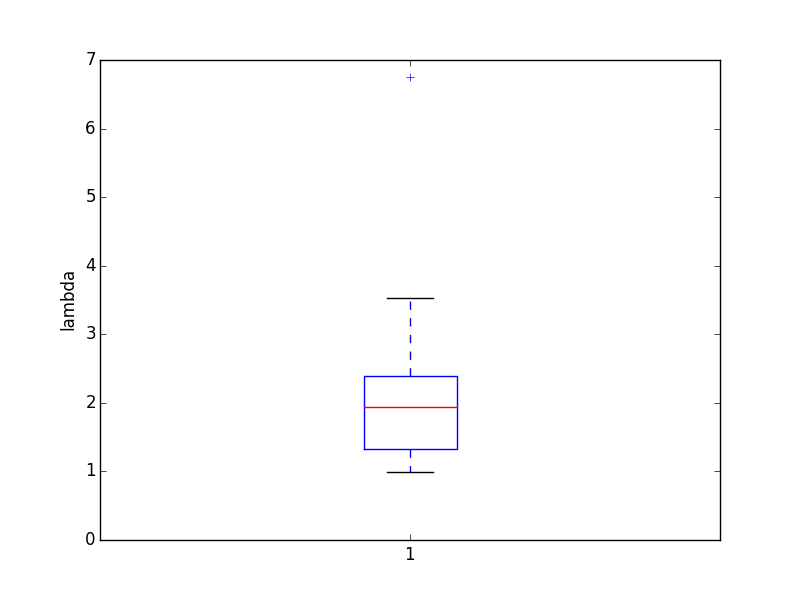
\includegraphics[scale=0.35]{figures/lambda_boxplot.png}
\end{figure}
The accuracy of Logistic models (for 16 participants, there are 16 models in 
total) on the training set yielded a median of 89.78\% (min=80.97\%, 
max=99.21\%). We also did the model evaluation using 10-fold cross-validation, 
they are still performing accuracies of a median of 89.86\% (min=79.92\%, 
max=98.45\%).


\subsection{Linear Regression on BOLD data}

The topic we are interested in exploring is whether loss aversion reflects 
the engagement of distinct emotional processes when potential gains and 
losses are considered. In the process, we want to explore the correlation 
between neural and behavioral loss aversion in whole brain analysis. We also 
want to try to identify the regions of brain that is more activated by this 
loss aversion activity.

Since we want to explore the correlation between neural and behavioral loss 
aversion, the second step is to find out the neural loss aversion. In order 
to find the neural loss aversion, we perform a linear regression on the BOLD 
data against the parametric gain values and the parametric loss values, as 
explained in our model section. While implementing the linear regression, we 
added linear and quadratic drift in our model. These drift terms are modeling 
for gradual drifts across the time series.

We are especially interested in the beta coefficients of our parametric gain 
and parametric loss regressors, which are the first two columns in our design 
matrix. By looking at the coefficient values, we can get a general idea of 
how potential gains and potential losses affect brain activation. By plotting 
heat maps for gain and loss coefficients, we can identify the areas that have 
large coefficients; these are the areas that the brain activation is highly 
connected to the potential gains and losses. We choose subject 2 to plot heat 
maps. We plot slices 2 to 31 from the third dimension of the brain (top to 
bottom). The red color is associated with large coefficients and blue color 
is associated with small coefficients.

From the gain and loss coefficients, we can also compute the neural loss 
aversion. This serves the next step of looking at the correlation between 
neural and behavioral loss aversion. The neural gain and loss coefficients 
were broadly distributed and spanned zero, so it is not possible to compute 
the ratio of loss to gain coefficients, nor does it make much sense. 
Therefore, we compute the neural loss aversion at every voxel by subtracting 
the slope of the gain response from the (negative) slope of the loss response. 
Again, we plot the heat maps for subject 2’s difference in gain and loss 
coefficients. With the neural loss aversion values calculated, we can explore 
how loss aversion affects brain activation when potential gains and losses are 
considered.

\begin{figure}[H]
    \centering
        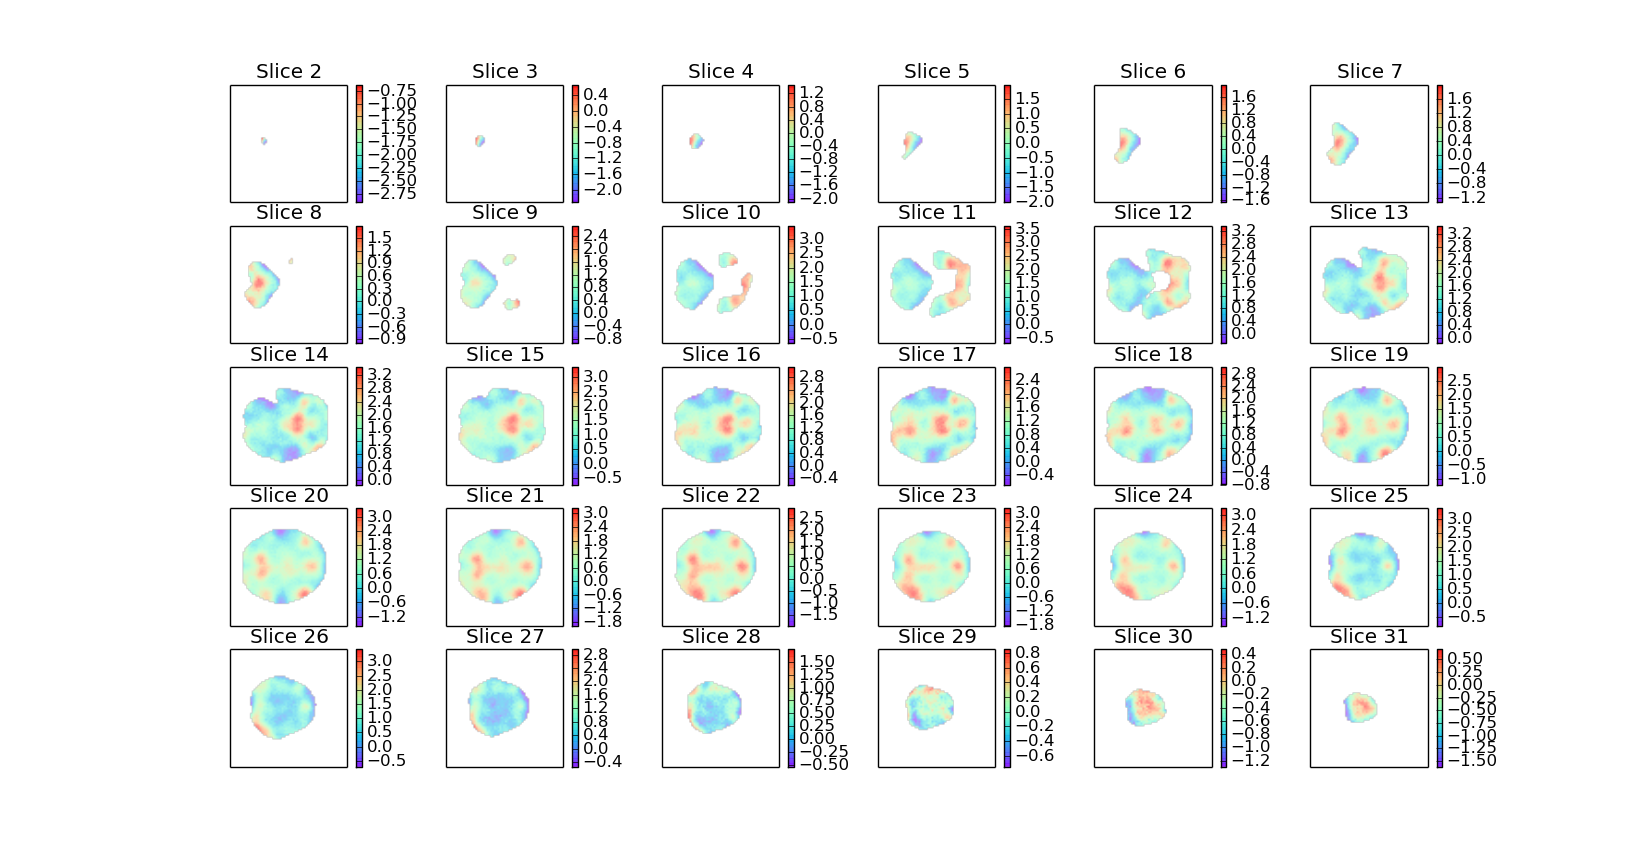
\includegraphics[scale=0.42]{figures/sub2gain_heatmap.png}
    \caption{Coefficients of the gain values for subject 2}
\end{figure}

\begin{figure}[H]
    \centering
        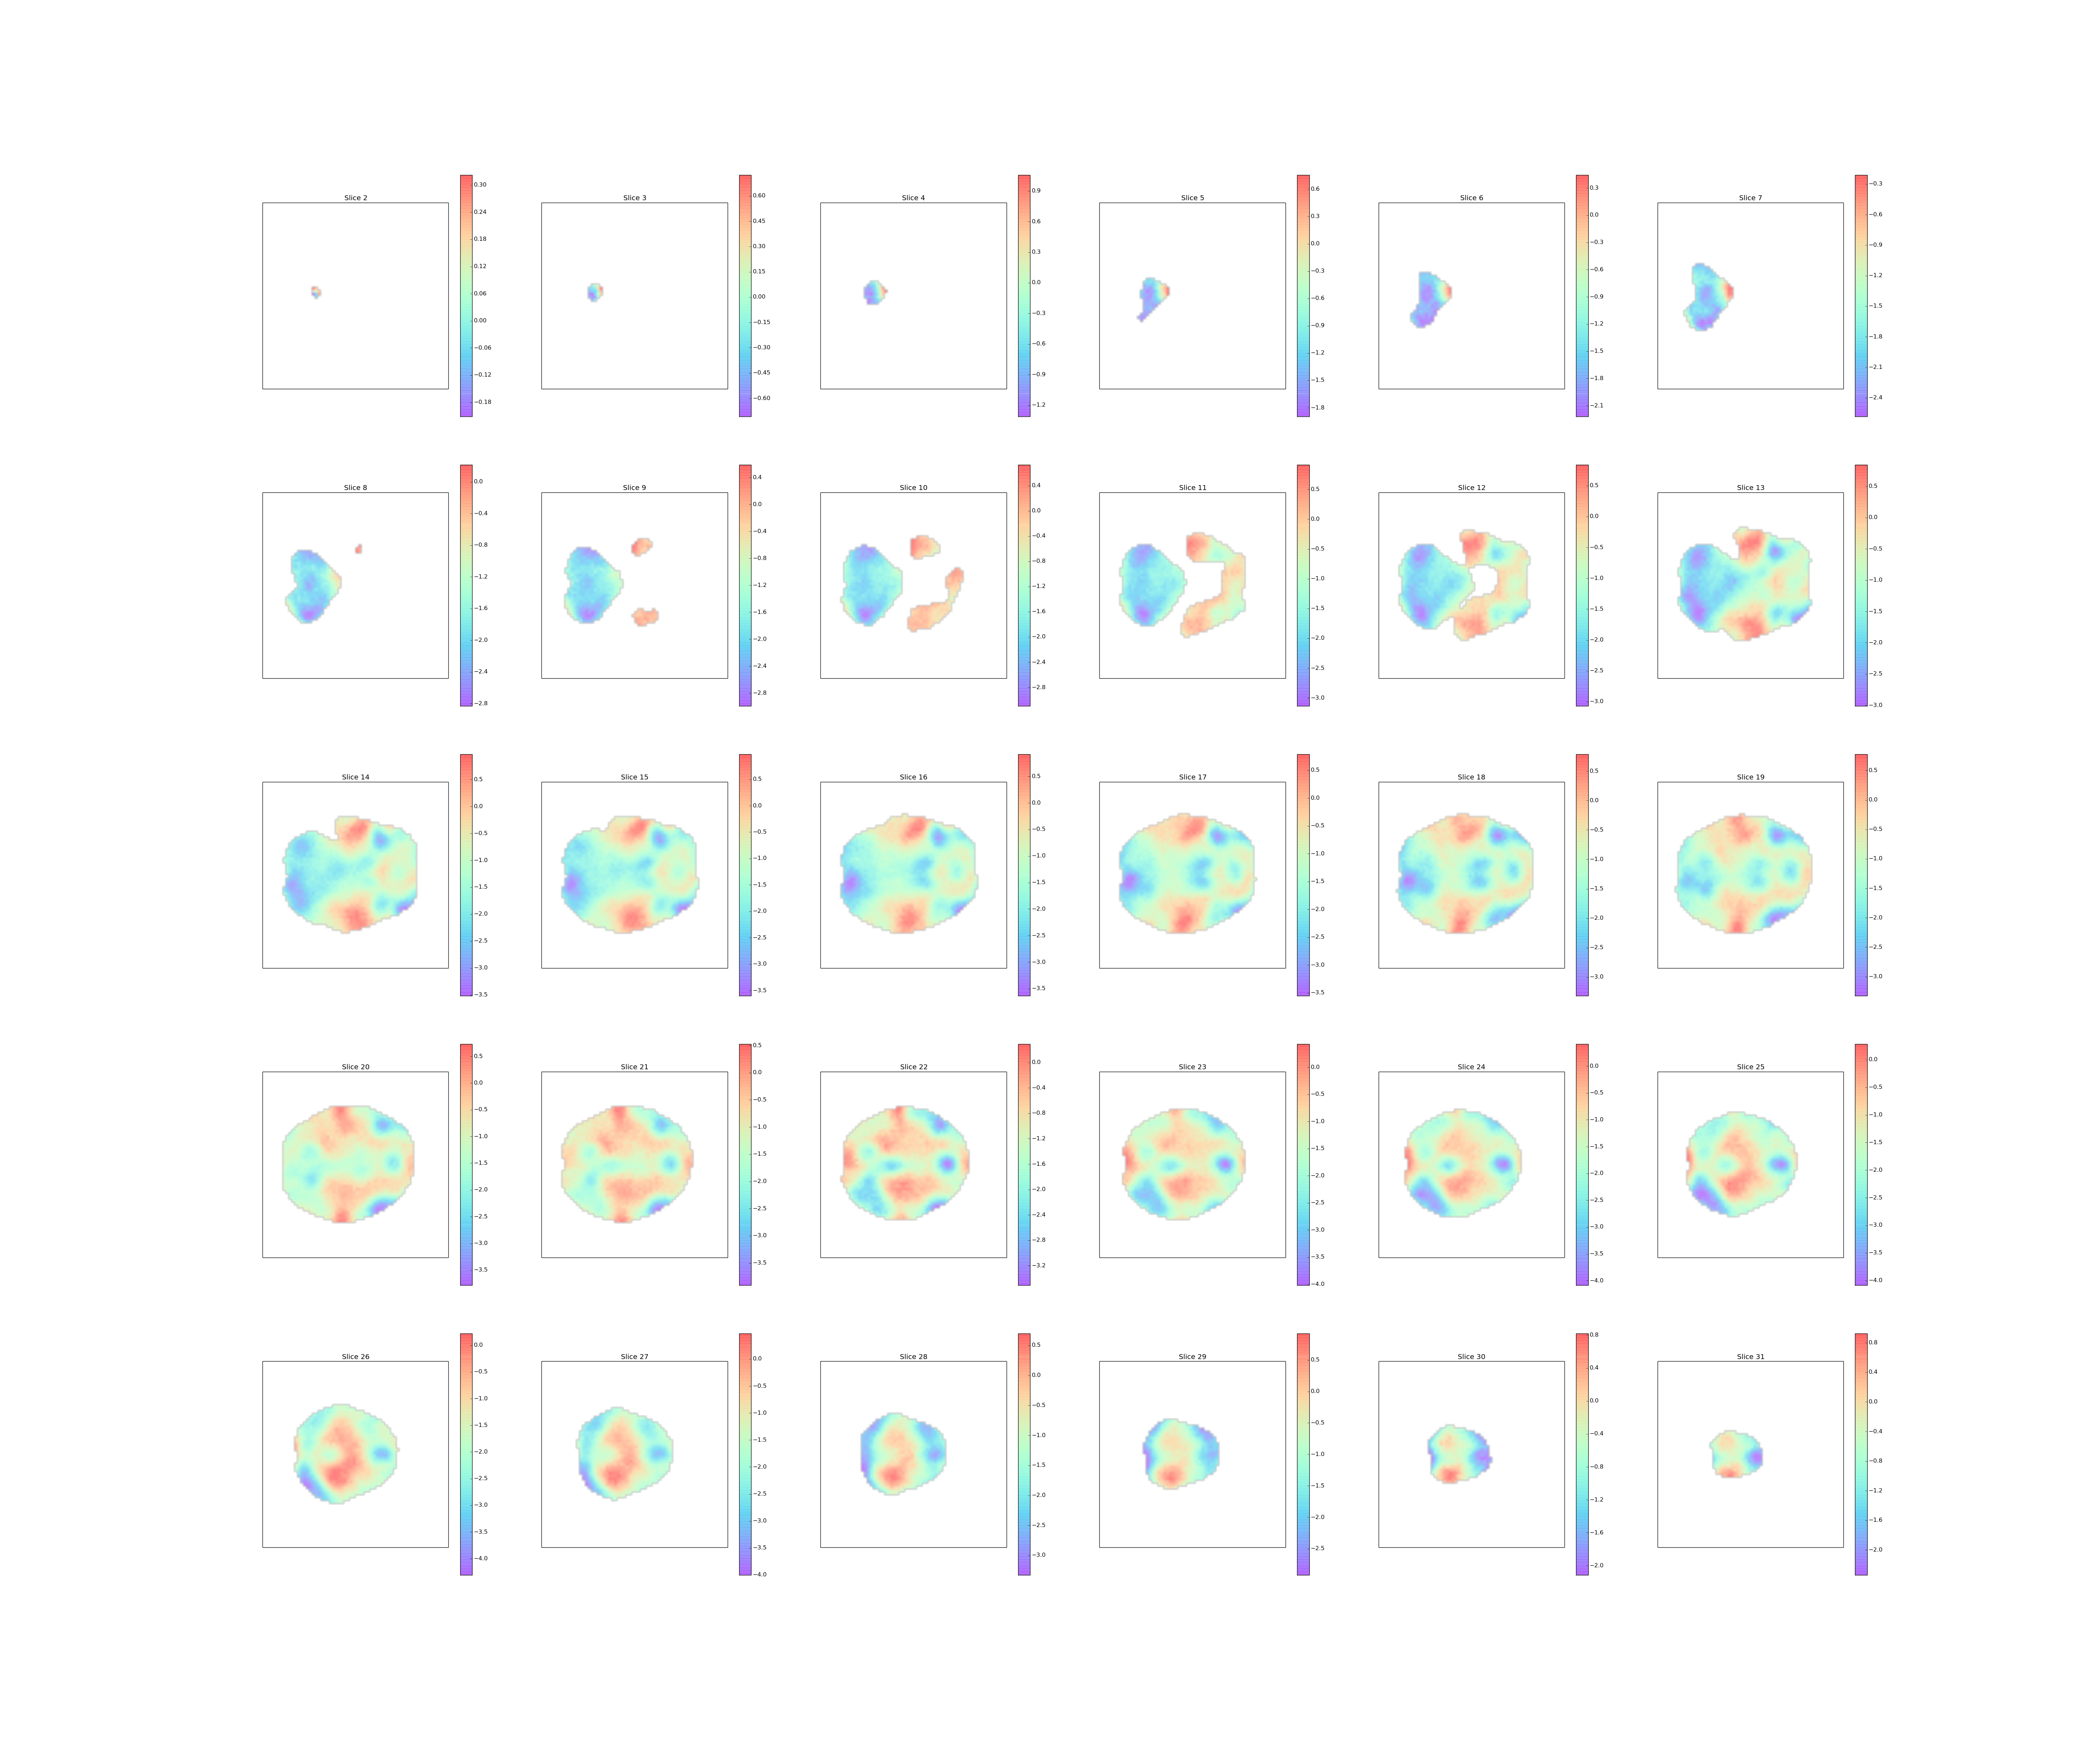
\includegraphics[scale=0.42]{figures/sub2loss_heatmap.png}
    \caption{Coefficients of the loss values for subject 2}
\end{figure}

\begin{figure}[H]
    \centering
        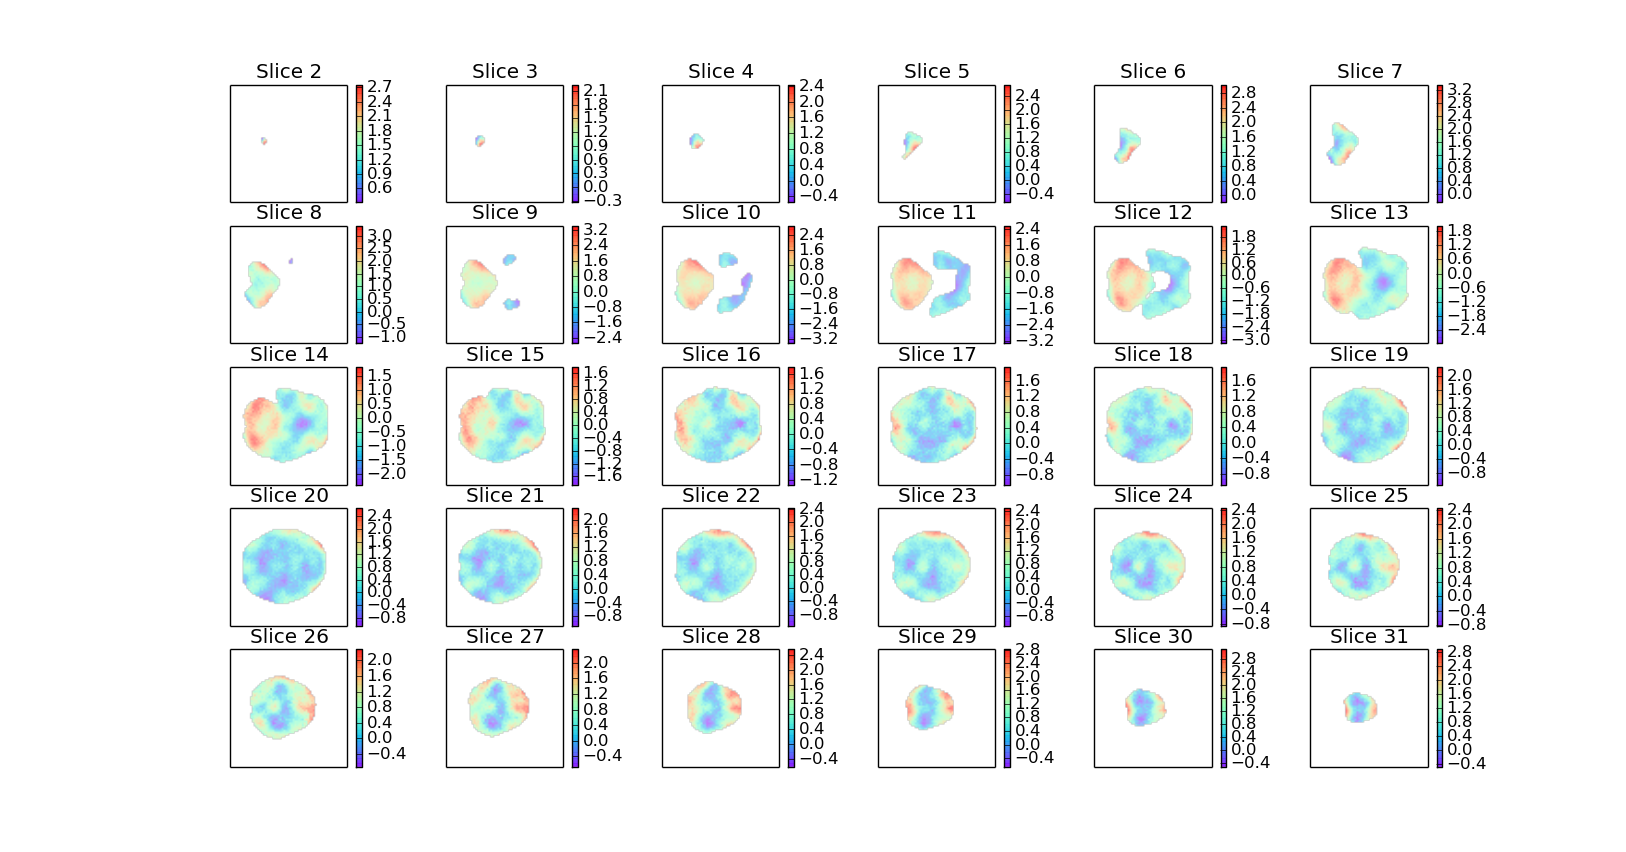
\includegraphics[scale=0.42]{figures/sub2diff_heatmap.png}
    \caption{Difference between gain and loss coefficients for subject 2}
\end{figure}

In the near future, we will calculate the p-values and/or t statistics for 
each voxel of each subject and subset all the voxels with significant 
coefficients. Then, we can produce heat maps of the t statistics for the gain 
and loss coefficients of each voxel. Plotting this will show us regions with 
significant parametric increase in fMRI signal to increasing potential gains 
and regions with significant parametric decrease to increasing potential 
losses. On one hand, we can perform linear regression assumption check in 
doing so; on the other hand, we can also see the coefficients in which regions 
are significant and thus have significant brain activation.


\subsection{Mixed-effects model on fMRI data}
First, we did the ANOVA test for each subject each voxels, grouping by runs. 
The high proportion of significant ANOVA F-test (after  Bonferroni correction 
under 0.05 significant level) shows that mixed effects model may perform well 
when collapsing three runs into one model. 
\begin{figure}[H]
\caption{Box plot of the proportion of significant ANOVA test}
    \centering
        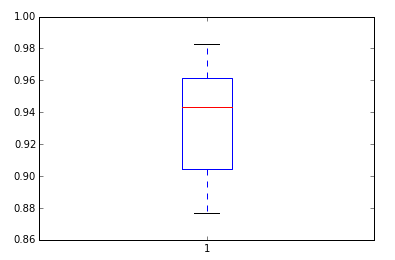
\includegraphics[scale=0.45]{figures/anova_prop.png}
\end{figure}
Following are the slices of coefficient of gain for subject 002. The 
mixed-effects model for each subject yielded a a median of 9.4\% (min=6.4\%, 
max=21.5\%) and 8.3\% (min=4.6\%, max=15.4\%) of proportion of significant 
coefficient for gain and loss separately. 
\begin{figure}[H]
\caption{heatmap of coefficient of gain for subject 002}
    \centering
        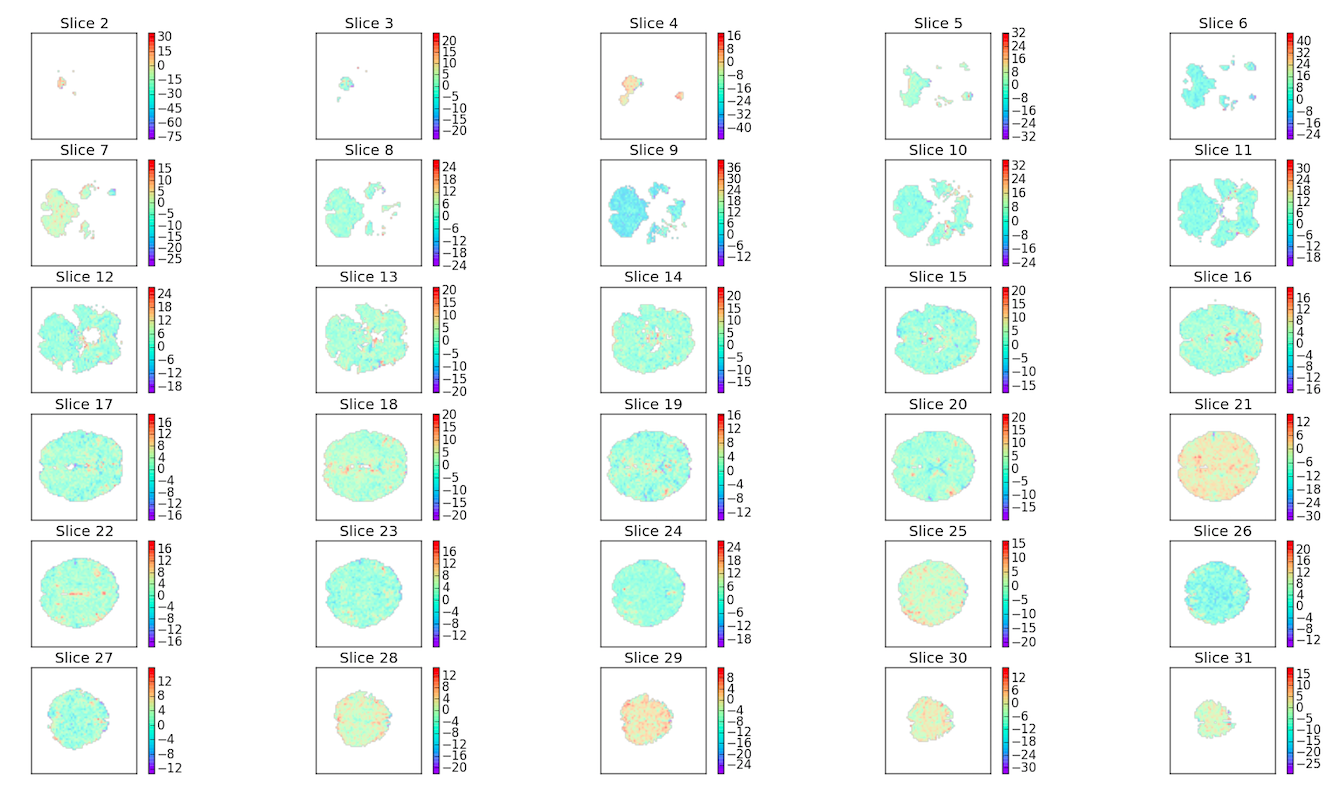
\includegraphics[scale=0.35]{figures/sub002_lme_beta_gain.png}
\end{figure}


